% ============================================================================
% Appendix: classical sampling of VQPM
% ============================================================================

\section{Classical sampling of VQPM}
\setcounter{equation}{0}
\renewcommand{\theequation}{\thesection\arabic{equation}}
\label{app:sampling}
For QUBO problems, everything VQPM measures can be generated by classical sampling. This appendix states this precisely (Appendix~\ref{app:classical}), compares the number of device shots with the number of classical draws (Appendix~\ref{app:shots}), uses the classical sampler to run VQPM up to $n=100$ (Appendix~\ref{app:large}), and derives the first-order form of the update and gives the details of the runs of Sec.~\ref{sec:update} (Appendices~\ref{app:flow} and~\ref{app:lockflow}). The notation is that of Appendix~\ref{app:theory}.

\subsection{Shot-by-shot simulation}
\label{app:classical}
\begin{proposition}[Shot-by-shot classical simulation]
\label{prop:classical}
Let $\mathcal{U}$ be diagonal and let the input have a computational-basis distribution $p$ that can be sampled classically, such as the product states of VQPM. Then one VQPM shot, the control bit $c$ together with all register bits $x$, has the distribution $\Pr(c=0,x)=p(x)w(x)$ and $\Pr(c=1,x)=p(x)(1-w(x))$. A classical algorithm samples it exactly: draw $x\sim p$ in $O(n)$ time, compute $E(x)$ and $\lambda(x)$ in $O(n^2)$, and output $c=0$ with probability $w(x)$. The same holds for $k$ coherent rounds: given $x$, the $k$ control outcomes are independent, each equal to $0$ with probability $w(x)$.
\end{proposition}
\begin{proof}
Each round multiplies the amplitude of $\ket{x}$ by $(1\pm e^{i\lambda(x)})/2$ for control outcome $0$ or $1$, whose squared moduli are $w(x)$ and $1-w(x)$. No amplitudes of different $x$ interfere, because $\mathcal{U}$ is diagonal and $x$ is measured in the computational basis.
\end{proof}

Consequently, VQPM for QUBO as defined here can be reproduced classically shot by shot, at $O(n^2)$ cost per shot and with the same number of shots, including its finite-shot locking decisions. It cannot by itself give a quantum speedup. An advantage would require a non-diagonal Hamiltonian, inputs whose distribution cannot be sampled classically, or coherent amplitude amplification of the post-selection in the $k$-round version, which can at most reduce the $1/Z_k$ repetitions of Eq.~\eqref{eq:app-survival} quadratically. We therefore present VQPM here as a heuristic whose convergence and locking behaviour we analyse, not as evidence of quantum advantage (Remark~\ref{rem:classical} and Sec.~\ref{sec:conclusion}).

\subsection{Number of shots: device and classical sampler}
\label{app:shots}
The sampler of Proposition~\ref{prop:classical} reproduces the shot statistics of the device exactly, so for any locking rule it needs at most as many draws as the device needs shots. The work per shot is of the same order. A device shot prepares the product state with $n$ $R_y$ gates, applies controlled-$\mathcal{U}$, which for a dense $Q$ takes one controlled phase gate per term of $E(x)$ ($n$ two-qubit and $n(n-1)/2$ three-qubit gates), and measures $n+1$ qubits. A classical draw takes $n+1$ random numbers and the $n(n+1)/2$ multiply-adds of $E(x)$.

The classical sampler can, however, use far fewer draws than the device, for two reasons. First, it knows $w(x)$, while a shot reveals only one Bernoulli bit of it, so it can drop the control bit and weight every draw by $w(x)$. Second, the input marginals $\pi_i$ are known exactly, since they set the $R_y$ angles, so $\mathbb{E}_p[x_i]=\pi_i$ can serve as a control variate. Together these give the estimate
\begin{equation}
\hat\pi_i'=\pi_i+\frac{\frac1N\sum_{s=1}^{N}\bigl(x^{(s)}_i-\pi_i\bigr)\bigl(w(x^{(s)})-\bar w\bigr)}{\bar w},\qquad \bar w=\frac1N\sum_{s=1}^{N}w(x^{(s)}),\quad x^{(s)}\sim p .
\label{eq:app-weighted}
\end{equation}
Write $a_i=x_i-\pi_i$ and $\Delta_i=\pi_i'-\pi_i$. To first order in $1/N$, the device's estimate from its accepted shots, as in the main text, has variance $\mathbb{E}_p[w\,(x_i-\pi_i')^2]/(NW^2)$. The device can lower this to $\mathbb{E}[(a_i(c-W)-\Delta_ic)^2]/(NW^2)$ by keeping the rejected shots and using the same control variate. Eq.~\eqref{eq:app-weighted} has variance $\mathbb{E}_p[(a_i(w-W)-\Delta_iw)^2]/(NW^2)$. The last is never larger than the device's control-variate estimate, because $c$ is $w(x)$ plus Bernoulli noise of variance $w(1-w)$, which adds $\mathbb{E}_p[(a_i-\Delta_i)^2w(1-w)]$. The size of the gap is set by the spread of $w$ under $p$, which is small because the phase map compresses all energies into a window narrower than $\pi/2$. Table~\ref{tab:app-shots} evaluates the three variances in every round of the paper-setting runs, for the worst unlocked qubit. Keeping the rejected shots and using the control variate saves the device a factor of about $10$. Eq.~\eqref{eq:app-weighted} needs at most $2\times10^{-3}$ of the device's shots in any round, and typically $10^{-5}$. Most of this gain comes from the control variate: weighting alone changes the variance only by a factor within $2\times10^{-3}$ of $W\approx0.9$. For the locking guarantee of Proposition~\ref{prop:threshold} with $p_{\mathrm{diff}}=0.01$, $\delta=0.05$ and $T=30$, the device needs $2.1$ to $2.2\times10^5$ shots per round with the post-selected estimate, or about $2\times10^4$ with the control variate, while the classical sampler reaches the same variance with fewer than $500$ draws per round. For comparison, rounding the marginals to three decimals, as in the main-text simulations, corresponds to a standard error of about $5\times10^{-4}$, which near $\pi_i'=1/2$ needs about $10^6$ post-selected shots per round on the device.

\begin{table}[ht]
\centering
\small
\caption{Shots per round on the paper-setting runs of Table~\ref{tab:app-locking} (100 instances per $n$, all rounds). Terms: number of terms of $E(x)$, which is the number of controlled phase gates per device shot and of multiply-adds per classical draw. Post-selected: device shots $M/W$ for the guarantee of Proposition~\ref{prop:threshold} ($p_{\mathrm{diff}}=0.01$, $\delta=0.05$, $T=30$, $M=2\ln(2nT/\delta)/p_{\mathrm{diff}}^2$), with the median $W$. The last two columns give the number of draws that reaches the same variance for the worst unlocked qubit, as a fraction of the post-selected count, median over rounds [largest]: the device keeping all shots with the control variate $\mathbb{E}_p[x_i]=\pi_i$, and the classical estimate of Eq.~\eqref{eq:app-weighted}.}
\label{tab:app-shots}
\begin{tabular}{rrcrcc}
\toprule
$n$ & terms & $W$, median [range] & post-selected & device, control variate & classical, Eq.~\eqref{eq:app-weighted} \\
\midrule
8 & 36 & 0.897 [0.797, 0.972] & $2.05\times10^5$ & 0.10 [0.20] & $3\times10^{-5}$ [$2.1\times10^{-3}$] \\
12 & 78 & 0.901 [0.817, 0.946] & $2.13\times10^5$ & 0.10 [0.18] & $5\times10^{-6}$ [$7.1\times10^{-4}$] \\
16 & 136 & 0.892 [0.829, 0.934] & $2.21\times10^5$ & 0.11 [0.17] & $7\times10^{-6}$ [$3.6\times10^{-4}$] \\
\bottomrule
\end{tabular}
\end{table}

For $k$ coherent rounds, weighting each draw by $w(x)^k$ instead of post-selecting already changes the variance by a factor of at most $\max_xw(x)^k=\cos^{2k}(\lambda_d/2)$, since $w^{2k}\le w^k\max_xw^k$. Weighting thus removes the eigenvalue factor of Eq.~\eqref{eq:app-survival}, which the device pays in repetitions. It does not remove the cost of finding the optimum by sampling from $p_0$: the effective sample size $NZ_k^2/Z_{2k}$ of the weighted sampler tends to $NA$ for large $k$, so from the uniform start it still needs about $2^n/|X^*|$ draws.

\subsection{Larger instances}
\label{app:large}
The estimate of Eq.~\eqref{eq:app-weighted} needs no $2^n$ state vector, so the VQPM loop can be run classically far beyond the $n\le20$ of the main text. With $N=2\times10^4$ draws per round its marginals agree with exact enumeration at $n=20$ to within $1.1\times10^{-4}$, well below the rounding unit $5\times10^{-4}$ of the main-text simulations. We ran 100 instances for each $n=20,30,\dots,100$ from the same family as above ($Q=G+G^T$, $G_{ij}\sim\mathcal N(0,1)$, seed $2026+n$), with the phase map of Eq.~\eqref{eq:phasemap} and the following stop rule: stop when the reference string $x_{\mathrm{ref}}$ reaches probability $1/2$ after the filter, or when a lock contradicts it. At $n=20$, $x_{\mathrm{ref}}$ is the exhaustive optimum. For $n\ge30$ it is the best of 32 simulated-annealing chains, each followed by 1-flip descent. All 32 chains returned the same energy in 100\% of the instances for $n\le30$, in 93 to 99\% for $n=40$ to $80$, and in 83 and 88\% for $n=90$ and $100$; at $n=20$ annealing found the exhaustive optimum every time.

\paragraph{The first round.} From the uniform start, expanding $w$ to first order around the phase $\bar\lambda$ of the mean energy, $w\approx w(\bar\lambda)-\tfrac12\sin\bar\lambda\,(\lambda-\bar\lambda)$, and using $\mathrm{Cov}(x_i,E)=g_i/4$ under the uniform distribution gives
\begin{equation}
D_i:=P_1-P_0\;\approx\;-\frac{\pi\sin\bar\lambda}{16\,S\cos^2(\bar\lambda/2)}\,g_i,\qquad g_i=Q_{ii}+\tfrac12\sum_{j\ne i}Q_{ij},
\label{eq:app-round1}
\end{equation}
where $g_i=\partial\bar E/\partial\pi_i$ at $\pi=1/2$ is the mean-field gradient of Appendix~\ref{app:sos}. Eq.~\eqref{eq:app-round1} is the first round of the first-order map of Appendix~\ref{app:flow}. The first round therefore moves every qubit against its mean-field gradient, by an amount proportional to $g_i/S$. For these instances $g_i$ has standard deviation $\sqrt{(n+7)/2}$ and $S\approx0.56\,n^2$, so $|D_i|$ shrinks like $n^{-3/2}$. Table~\ref{tab:app-round1} and Fig.~\ref{fig:app-large}(a) confirm this: the median $|D_i|$ falls from $1.6\times10^{-3}$ at $n=20$ to $1.4\times10^{-4}$ at $n=100$, with fitted exponents $-1.50$ for the median and $-1.40$ for the largest $|D_i|$. Eq.~\eqref{eq:app-round1} is within 3\% of the sampled values and has the same sign for 99\% of the qubits. At every $n$, about 78\% of the round-1 signs agree with $x_{\mathrm{ref}}$, while the qubit with the largest $|D_i|$ agrees in 98 to 100\% of the instances.

\paragraph{Shots needed to see the first round.} A device estimates $D_i$ from post-selected shots with standard deviation $1/\sqrt{NW}$, so resolving the median $|D_i|$ at three standard deviations takes $N=9/(WD^2)$ shots. This grows like $n^3$: from $3.9\times10^6$ at $n=20$ to $5.3\times10^8$ at $n=100$, with fitted exponent $3.01$ (Table~\ref{tab:app-round1}, Fig.~\ref{fig:app-large}(b)). The shots can be spread over several rounds, but not saved: over $t$ rounds the drift adds up to about $tD$ and the noise only to $\sqrt t$ times its one-round size, so the total is still about $9/(WD^2)$. The classical estimate of Eq.~\eqref{eq:app-weighted} has standard deviation about $\sigma_w/(W\sqrt N)$, where $\sigma_w$ is the spread of $w$ under the input distribution, and needs $9\sigma_w^2/(W^2D^2)$ draws. Since $\sigma_w$ falls like $1/n$ (fitted exponent $-0.99$), this grows only like $n$: from $5.2\times10^2$ to $2.9\times10^3$ (exponent $1.03$).

\begin{table}[ht]
\centering
\small
\caption{Round 1 from the uniform start, 100 instances per $n$, $2\times10^5$ draws each with Eq.~\eqref{eq:app-weighted}. Median and largest: median over instances of the per-instance median and largest $|D_i|$, $D_i=P_1-P_0$. Erased: qubits with $|D_i|<10^{-3}$, whose marginal rounds back to $0.500$ at three decimals; no qubit had $|D_i|\ge0.01$ at any $n\ge20$. Agrees: share of the signs of $D_i$ that agree with $x_{\mathrm{ref}}$. Device and classical: draws per round that resolve the median $|D_i|$ at three standard deviations, $9/(WD^2)$ post-selected shots and $9\sigma_w^2/(W^2D^2)$ draws of Eq.~\eqref{eq:app-weighted}.}
\label{tab:app-round1}
\begin{tabular}{rccccrr}
\toprule
$n$ & median $|D_i|$ & largest $|D_i|$ & erased & agrees & device & classical \\
\midrule
20 & $1.6\times10^{-3}$ & $5.1\times10^{-3}$ & 32\% & 78\% & $3.9\times10^6$ & 520 \\
30 & $8.3\times10^{-4}$ & $2.9\times10^{-3}$ & 57\% & 78\% & $1.5\times10^7$ & 870 \\
40 & $5.5\times10^{-4}$ & $2.0\times10^{-3}$ & 76\% & 79\% & $3.4\times10^7$ & 1140 \\
50 & $4.0\times10^{-4}$ & $1.5\times10^{-3}$ & 90\% & 78\% & $6.4\times10^7$ & 1380 \\
60 & $3.0\times10^{-4}$ & $1.1\times10^{-3}$ & 98\% & 78\% & $1.2\times10^8$ & 1680 \\
70 & $2.4\times10^{-4}$ & $9.0\times10^{-4}$ & 100\% & 79\% & $1.8\times10^8$ & 1960 \\
80 & $2.0\times10^{-4}$ & $7.4\times10^{-4}$ & 100\% & 78\% & $2.7\times10^8$ & 2250 \\
90 & $1.7\times10^{-4}$ & $6.3\times10^{-4}$ & 100\% & 78\% & $3.9\times10^8$ & 2530 \\
100 & $1.4\times10^{-4}$ & $5.4\times10^{-4}$ & 100\% & 78\% & $5.3\times10^8$ & 2850 \\
\bottomrule
\end{tabular}
\end{table}

\paragraph{Paper settings and a finite-shot device.} We first ran the loop with $p_{\mathrm{diff}}=0.01$ and at most 30 rounds, as in the main text, in two versions (Table~\ref{tab:app-large}).
\begin{itemize}
\item \emph{Marginals rounded to three decimals}, as in the main-text simulations. Rounding erases most of the round-1 signal, and the rounded marginals then repeat unchanged, so the run stalls. All runs stall for $n\ge60$. The share that stalls in round 1 with nothing locked rises from 27\% at $n=60$ to 74\% at $n=70$ and 99 to 100\% for $n\ge80$. Only 11\% of the runs reach $x_{\mathrm{ref}}$ at $n=20$, and none do for $n\ge30$. If a run that stalls with $x_{\mathrm{ref}}$ as its most probable string is also counted as a success, as in Sec.~\ref{sec:comparison}, the share is 26\% at $n=20$, 3\% at $n=30$ and at most 1\% for $n\ge40$.
\item \emph{A device with $2\times10^5$ shots per round} (post-selected estimate, three decimals). The shot noise in $\hat D_i$ has standard deviation $1/\sqrt{MW}\approx2.4\times10^{-3}$, which exceeds the largest round-1 difference for $n\ge40$. The locks then follow the noise: 75\% of the runs end in a wrong lock at $n=20$, 98\% at $n=30$ and all of them for $n\ge40$. In 33\% (at $n=20$) to 93\% (at $n=100$) of the runs, the same loop without rounding or shot noise made no wrong lock in the same 30 rounds.
\end{itemize}

\begin{table}[ht]
\centering
\small
\caption{VQPM with the main-text settings ($p_{\mathrm{diff}}=0.01$, at most 30 rounds), 100 instances per $n$. Reached: runs in which $x_{\mathrm{ref}}$ reaches probability $1/2$. Wrong lock: runs stopped by a lock that contradicts $x_{\mathrm{ref}}$. Stalled: rounded marginals repeat unchanged.}
\label{tab:app-large}
\begin{tabular}{r ccc cc}
\toprule
 & \multicolumn{3}{c}{three decimals} & \multicolumn{2}{c}{device, $2\times10^5$ shots} \\
\cmidrule(lr){2-4}\cmidrule(lr){5-6}
$n$ & reached & wrong lock & stalled & reached & wrong lock \\
\midrule
20 & 11\% & 39\% & 50\% & 18\% & 75\% \\
30 & 0\% & 53\% & 42\% & 1\% & 98\% \\
40 & 0\% & 20\% & 70\% & 0\% & 100\% \\
50 & 0\% & 2\% & 94\% & 0\% & 100\% \\
60 & 0\% & 0\% & 100\% & 0\% & 100\% \\
70 & 0\% & 0\% & 100\% & 0\% & 100\% \\
80 & 0\% & 0\% & 100\% & 0\% & 100\% \\
90 & 0\% & 0\% & 100\% & 0\% & 100\% \\
100 & 0\% & 0\% & 100\% & 0\% & 100\% \\
\bottomrule
\end{tabular}
\end{table}

\begin{figure}[ht]
\centering
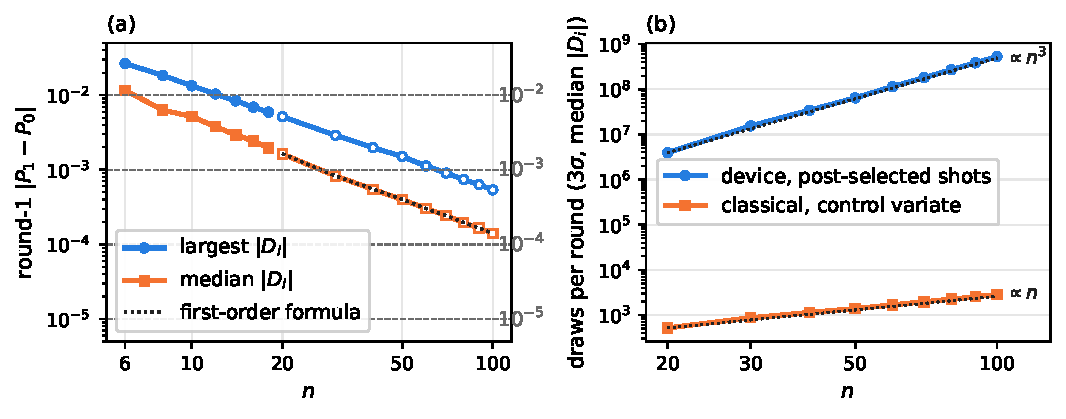
\includegraphics[width=\linewidth]{app_large_n}
\caption{(a) Round-1 $|P_1-P_0|$ from the uniform start: largest and median over the qubits, median over 100 instances per $n$. Filled markers: exact enumeration ($n\le18$); open markers: sampled with Eq.~\eqref{eq:app-weighted} ($n\ge20$); dotted: Eq.~\eqref{eq:app-round1}. Dashed lines: thresholds $10^{-2}$ to $10^{-5}$; $10^{-3}$ is also the smallest difference that survives rounding to three decimals. (b) Draws per round that resolve the median $|D_i|$ at three standard deviations, for the device's post-selected estimate and the classical estimate of Eq.~\eqref{eq:app-weighted}, with reference slopes $n^3$ and $n$. The threshold sweep without rounding is in Fig.~\ref{fig:app-flow}.}
\label{fig:app-large}
\end{figure}

\subsection{The product-state map without locking}
\label{app:flow}
Every VQPM run mixes two mechanisms: the product-state update of Eq.~\eqref{eq:app-vqpm} and locking. This section studies the update alone, with exact marginals and without locking or rounding; Appendix~\ref{app:lockflow} then adds locking. For $n\ge30$ the exact map cannot be iterated, but the phases of the strings that carry the probability lie close together, and to first order in their spread the map has a closed form.

\begin{proposition}[First-order form of the product-state map]
\label{prop:meanfield}
Let $J$ be the coupling matrix, $J_{ij}=J_{ji}=Q_{ij}$ for $i<j$ and $J_{ii}=0$. Let $\bar E(\pi)=\mathbb{E}_{p_\pi}[E]=\sum_iQ_{ii}\pi_i+\frac12\pi^TJ\pi$ be the mean energy of the product state, $g_i(\pi)=\partial\bar E/\partial\pi_i=Q_{ii}+\sum_jJ_{ij}\pi_j$ its gradient, and $\bar\lambda=\frac\pi4+\frac\pi4\bar E(\pi)/S$ the phase of the mean energy. To first order in the spread of the phases under $p_\pi$, Eq.~\eqref{eq:app-vqpm} is
\begin{equation}
\pi_i'=\pi_i-\eta(\pi)\,\pi_i(1-\pi_i)\,g_i(\pi),\qquad\eta(\pi)=\frac{\pi\sin\bar\lambda}{8S\cos^2(\bar\lambda/2)}.
\label{eq:app-mf}
\end{equation}
\end{proposition}
\begin{proof}
Let $\bar w=\cos^2(\bar\lambda/2)$. Since $\lambda(x)-\bar\lambda=\frac{\pi}{4S}(E(x)-\bar E)$, to first order $w(x)=\bar w-\frac{\pi\sin\bar\lambda}{8S}(E(x)-\bar E)$. Then $W=\bar w$, because $\mathbb{E}_{p_\pi}[E-\bar E]=0$, and $\sum_{x:\,x_i=1}p_\pi(x)w(x)=\pi_i\bigl[\bar w-\frac{\pi\sin\bar\lambda}{8S}(\mathbb{E}[E\mid x_i=1]-\bar E)\bigr]$. As $\bar E$ is affine in each $\pi_i$, $\mathbb{E}[E\mid x_i=1]$ is $\bar E$ evaluated at $\pi_i=1$, so $\mathbb{E}[E\mid x_i=1]-\bar E=(1-\pi_i)\,g_i$. Dividing by $W$ gives Eq.~\eqref{eq:app-mf}.
\end{proof}

The neglected terms are smaller than the kept ones by a factor of order the spread of the phases, $\frac{\pi}{4S}\,\mathrm{sd}_{p_\pi}(E)$. On our instances this is about $0.6/n$ at the uniform start, and it falls as the marginals leave $1/2$. Iterated from the uniform start until the marginals settle, Eq.~\eqref{eq:app-mf} ends at the same string as the exact map in 59 of 60 instances at $n=8$ and $12$, after the same median number of rounds to within 4\%. Three consequences follow.
\begin{itemize}
\item \emph{A gradient method.} In the logits $\theta_i=\ln[\pi_i/(1-\pi_i)]$, Eq.~\eqref{eq:app-mf} reads $\theta_i'=\theta_i-\eta\,g_i+O(\eta^2g_i^2)$, the gradient method of Sec.~\ref{sec:gradient}. Proposition~\ref{prop:monotone} is its exact counterpart: $W\approx\cos^2(\bar\lambda/2)$ grows as $\bar E$ falls.
\item \emph{Step size.} At $\bar\lambda\approx\pi/4$, $\eta\approx0.33/S$, and $S\approx0.56\,n^2$ on our instances. From the uniform start, round 1 gives $D_i=2\pi_i'-1=-\eta g_i/2$, which is Eq.~\eqref{eq:app-round1}.
\item \emph{End points.} At a vertex $x$, $(1-2x_i)\,g_i(x)=E(x\oplus e_i)-E(x)$, so a small deviation of coordinate $i$ is multiplied by $1-\eta\,[E(x\oplus e_i)-E(x)]$ per round. This is the first-order form of $r_i$ in Proposition~\ref{prop:stability}, and the stable vertices are again the strict 1-flip local minima. The Hessian of $\bar E$ is $J$, which has zero trace, so every interior stationary point is a saddle and the iteration ends at a vertex. We call this vertex the end point $x_\infty$.
\end{itemize}

\paragraph{Near the centre: from $D_i$ to the couplings.} Write $\pi=\frac12+u$, $g^0=g(\frac12)$ and $\eta_0=\eta(\frac12)$. To first order in $u$, Eq.~\eqref{eq:app-mf} is linear, $u'=u-\frac{\eta_0}{4}(g^0+Ju)$, so from $u=0$
\begin{equation}
u(t)=-\bigl(I-B^t\bigr)J^{-1}g^0=-\sum_k\frac{1-a_k^t}{\mu_k}\,(v_k^Tg^0)\,v_k,\qquad B=I-\frac{\eta_0}{4}J,\quad a_k=1-\frac{\eta_0\mu_k}{4},
\label{eq:app-linear}
\end{equation}
where $\mu_k$ and $v_k$ are the eigenvalues and unit eigenvectors of $J$. With $\tau=4/(\eta_0|\mu_{\min}|)$, the marginals pass through two regimes.
\begin{itemize}
\item For $t\ll\tau$, $(1-a_k^t)/\mu_k\approx\eta_0t/4$ and $u(t)\approx-\frac{\eta_0t}{4}\,g^0=\frac t2\,D$. Every qubit keeps moving in the direction of its round-1 difference $D_i$, the sign of its gradient at the centre.
\item For $t\gtrsim\tau$, the components along eigenvectors with $\mu_k>0$ level off at $-(v_k^Tg^0)/\mu_k$, while those with $\mu_k<0$ grow like $(1+\eta_0|\mu_k|/4)^t$. The marginals turn toward the eigenvectors of $J$ with the most negative eigenvalues, with signs set by $g^0$.
\end{itemize}
This is the power iteration of the product state described in Sec.~\ref{sec:couplings}, with the linearized iteration matrix $B$. On our instances $J$ is a Wigner matrix with entry variance 2, so $\mu_{\min}\approx-2\sqrt{2n}$ and $\tau\approx2.5\,n^{3/2}$ for large $n$. The measured median of $\tau$ grows from 275 rounds at $n=20$ to 2\,610 at $n=100$, or $3.1$ to $2.6\,n^{3/2}$ (Table~\ref{tab:app-flow}). The linear regime ends when the $|u_i|$ approach $\frac12$; the factor $\pi_i(1-\pi_i)$ then slows the coordinates near 0 and 1, and the map settles at its end point.

\paragraph{Where the unlocked map goes.} Table~\ref{tab:app-flow} gives the end points of the unlocked runs of Sec.~\ref{sec:unlocked}, with the overlap $m(t)$ of Eq.~\eqref{eq:overlap}. Every run that settled ended at a strict 1-flip local minimum, and no run ended below $x_{\mathrm{ref}}$. The runs that miss level off at an overlap of about $0.7$ to $0.85$. The median run settles after 54 to 98 times $S$ rounds, and $x_{\mathrm{ref}}$ first reaches probability $1/2$ after $2.0\times10^3$ rounds at $n=20$ and $1.6\times10^5$ at $n=100$. Between 1 and 20 runs per $n$ were still moving after $3\times10^6$ rounds, close to a saddle; for them the end point is the nearest vertex.

\begin{table}[ht]
\centering
\small
\caption{The unlocked product-state map, Eq.~\eqref{eq:app-mf}, from the uniform start until every marginal is within $10^{-3}$ of a stable vertex (at most $3\times10^6$ rounds), 100 instances per $n$. $\tau=4/(\eta_0|\mu_{\min}(J)|)$ of Eq.~\eqref{eq:app-linear}, median. Misses: runs that end elsewhere than $x_{\mathrm{ref}}$, with their median distance in bits and median energy gap $(E-E_{\mathrm{ref}})/|E_{\mathrm{ref}}|$. Settle: median rounds until the run settles. $\Pr(x_{\mathrm{ref}})\ge\frac12$: median round in which $x_{\mathrm{ref}}$ first reaches probability $1/2$ after the filter, over the runs in which it does. Still moving: runs not settled after $3\times10^6$ rounds.}
\label{tab:app-flow}
\begin{tabular}{rrcccrrr}
\toprule
 & & & \multicolumn{2}{c}{misses} & & & \\
\cmidrule(lr){4-5}
$n$ & $\tau$ & ends at $x_{\mathrm{ref}}$ & bits & gap & settle & $\Pr(x_{\mathrm{ref}})\ge\frac12$ & still moving \\
\midrule
20 & 275 & 73\% & 3 & 1.3\% & 13\,714 & 1\,982 & 1 \\
30 & 475 & 58\% & 4 & 1.3\% & 44\,762 & 6\,572 & 3 \\
40 & 704 & 53\% & 4 & 0.9\% & 60\,400 & 11\,937 & 6 \\
50 & 966 & 48\% & 5 & 0.8\% & 106\,826 & 19\,790 & 5 \\
60 & 1\,250 & 41\% & 5 & 0.9\% & 165\,967 & 28\,992 & 6 \\
70 & 1\,557 & 34\% & 6 & 0.7\% & 182\,482 & 46\,472 & 8 \\
80 & 1\,894 & 38\% & 7 & 0.7\% & 275\,060 & 69\,658 & 15 \\
90 & 2\,256 & 19\% & 7 & 0.6\% & 359\,390 & 170\,479 & 20 \\
100 & 2\,610 & 24\% & 7.5 & 0.6\% & 563\,404 & 155\,226 & 20 \\
\bottomrule
\end{tabular}
\end{table}


\subsection{What locking adds}
\label{app:lockflow}
This section gives the details of the locked runs of Sec.~\ref{sec:locksigns}. Each run continues until every qubit is locked or the free ones have settled at a vertex that is stable for them.

\paragraph{The sign that a lock reads.} Table~\ref{tab:app-read} follows the unlocked map and records, for each threshold, the sign of every qubit in the round in which it first passes the threshold; Fig.~\ref{fig:app-flow}(c) plots the same shares. At $n=100$ the thresholds are passed in round 1 from $10^{-4}$ down, and after a median of 8 rounds at $10^{-3}$, 72 rounds at $10^{-2}$ and 1\,390 rounds at $0.2$, about $0.003\tau$, $0.03\tau$ and $0.5\tau$. Eq.~\eqref{eq:app-linear} predicts 97 to 100\% of all signs read and 94\% of those that differ from $D_i$, so the turn is the one toward the low eigenvectors of $J$. From $10^{-3}$ to $0.2$, the share of signs that agree with the unlocked end point rises from 81 to 94\%, and the share that agree with $x_{\mathrm{ref}}$ from 79 to 90\%: a larger threshold reads the signs later and closer to where the unlocked map ends.

\begin{table}[ht]
\centering
\small
\caption{Signs that locking reads, on the unlocked map at $n=100$ (100 instances). For each threshold: the sign of $2\pi_i-1$ in the round in which $|2\pi_i-1|$ first exceeds it, compared with the sign of the round-1 difference $D_i$, with the sign of the linear prediction $u_i(t)$ of Eq.~\eqref{eq:app-linear} in the same round, with the unlocked end point $x_\infty$ and with $x_{\mathrm{ref}}$, as shares of all qubits. Round: median over instances of the per-instance median round, in units of $\tau$ (median $\tau=2\,610$). At $n=20$ to $90$ the shares are within about 2 points of these.}
\label{tab:app-read}
\begin{tabular}{lccccc}
\toprule
 & & \multicolumn{4}{c}{sign read agrees with} \\
\cmidrule(lr){3-6}
$p_{\mathrm{diff}}$ & round$/\tau$ & $D_i$ & $u_i(t)$ & $x_\infty$ & $x_{\mathrm{ref}}$ \\
\midrule
$10^{-6}$ & round 1 & 100\% & 100\% & 80\% & 78\% \\
$10^{-4}$ & round 1 & 99.5\% & 100\% & 80\% & 78\% \\
$10^{-3}$ & 0.003 & 98\% & 100\% & 81\% & 79\% \\
$10^{-2}$ & 0.03 & 95\% & 99.8\% & 84\% & 82\% \\
$0.05$ & 0.14 & 90\% & 99\% & 89\% & 86\% \\
$0.1$ & 0.27 & 87\% & 98\% & 91\% & 88\% \\
$0.15$ & 0.41 & 85\% & 98\% & 93\% & 89\% \\
$0.2$ & 0.54 & 84\% & 97\% & 94\% & 90\% \\
\bottomrule
\end{tabular}
\end{table}

\paragraph{Success and rounds.} Table~\ref{tab:app-lockflow} and Fig.~\ref{fig:app-flow}(b, d) give the outcome of the locked runs. Below $10^{-2}$ the share of runs that reach $x_{\mathrm{ref}}$ drops quickly: at $n=20$ it is 15\% at $10^{-3}$ and 2\% at $10^{-4}$. The thresholds $0.05$ to $0.2$ gain at most 7 points over $10^{-2}$. At $p_{\mathrm{diff}}=0.2$, of the 1.1 wrong locks per run at $n=20$ and 7.8 at $n=100$, 0.7 and 3.4 also disagree with the unlocked end point $x_\infty$; of the instances in which the unlocked map ends at $x_{\mathrm{ref}}$, the run with $p_{\mathrm{diff}}=0.2$ still passes in 77\% at $n=20$ and 12\% at $n=100$. For $p_{\mathrm{diff}}\ge10^{-2}$ the number of rounds grows like $n^{1.9}$ to $n^{2.0}$, as $S$ does.


\paragraph{Check against sampled VQPM.} Table~\ref{tab:app-sweep} repeats the locked runs with sampled marginals: exact at $n=20$, and estimated with Eq.~\eqref{eq:app-weighted} for $n\ge30$, with $5\times10^4$ draws per round for $p_{\mathrm{diff}}\ge10^{-3}$ and $2\times10^5$ below. These runs use the stop rule of Appendix~\ref{app:large} and a budget of $\lceil1.5\,n^{3/2}\rceil$ rounds, which ran out in at most 1\% of them. On whether a run reaches $x_{\mathrm{ref}}$, sampled VQPM and Eq.~\eqref{eq:app-mf} agree on 99.0\% of the instances at $p_{\mathrm{diff}}=10^{-2}$, 98.3\% at $10^{-3}$, and all of them at $10^{-4}$ and $10^{-5}$. The table also lists the share of qubits that lock in round 1: 63 to 97\% at $10^{-4}$, and all of them from $10^{-6}$ down. For $n\ge30$ the sampled $\hat D_i$ has a standard deviation of about $2\times10^{-5}$ at $n=30$ and $6\times10^{-6}$ at $n=100$, so thresholds of $10^{-5}$ and below lie at or under the sampling noise there. This does not change the outcome, which is the same at $n=20$, where the marginals are exact, and in the first-order map, which has no noise.

\begin{table}[ht]
\centering
\small
\setlength{\tabcolsep}{4pt}
\caption{Sampled VQPM without rounding for a range of locking thresholds (exact marginals at $n=20$, Eq.~\eqref{eq:app-weighted} for $n\ge30$), 100 instances per $n$, at most $\lceil1.5\,n^{3/2}\rceil$ rounds, stop rule of Appendix~\ref{app:large} with $x_{\mathrm{ref}}$. It checks the first-order runs of Table~\ref{tab:app-lockflow}. Reached: runs in which $x_{\mathrm{ref}}$ reaches probability $1/2$; all other runs end in a wrong lock, except at most 1\% that use up the budget. Locked in round 1: share of the qubits locked in the first round.}
\label{tab:app-sweep}
\begin{tabular}{r cccc cccc}
\toprule
 & \multicolumn{4}{c}{reached $x_{\mathrm{ref}}$, $p_{\mathrm{diff}}=$} & \multicolumn{4}{c}{locked in round 1, $p_{\mathrm{diff}}=$} \\
\cmidrule(lr){2-5}\cmidrule(lr){6-9}
$n$ & $10^{-2}$ & $10^{-3}$ & $10^{-4}$ & $\le10^{-5}$ & $10^{-3}$ & $10^{-4}$ & $10^{-5}$ & $\le10^{-6}$ \\
\midrule
20 & 53\% & 15\% & 2\% & 0\% & 67\% & 97\% & 100\% & 100\% \\
30 & 29\% & 13\% & 0\% & 0\% & 43\% & 93\% & 99\% & 100\% \\
40 & 25\% & 13\% & 0\% & 0\% & 24\% & 91\% & 99\% & 100\% \\
50 & 19\% & 12\% & 0\% & 0\% & 10\% & 86\% & 99\% & 100\% \\
60 & 14\% & 11\% & 0\% & 0\% & 2\% & 83\% & 98\% & 100\% \\
70 & 5\% & 4\% & 0\% & 0\% & 0\% & 78\% & 97\% & 100\% \\
80 & 8\% & 6\% & 0\% & 0\% & 0\% & 73\% & 97\% & 100\% \\
90 & 3\% & 2\% & 0\% & 0\% & 0\% & 69\% & 97\% & 100\% \\
100 & 3\% & 3\% & 0\% & 0\% & 0\% & 63\% & 96\% & 100\% \\
\bottomrule
\end{tabular}
\end{table}
